\section{Preliminaries}
\subsection{Polygonal Chains}

Given are two polygonal chains $P$ and $Q$. A polygonal chain is defined by a list of points, sorted by order of the chain, ascending from beginning to end. The first point of the list is the start of the polygonal curve and the last point of the list is the end of the polygonal curve. This order implies the direction of the directional polygonal curve.

$P$ and $Q$ are polygonal chains consisting of $n$ and $m$ points respectively.

$$P_{points} = [P_1, P_2, …, P_n]$$
$$Q_{points} = [Q_1, Q_2, …, Q_m]$$

Points of P and Q are expressed as vectors:

$$P_{i} = \begin{pmatrix}x_{Pi} \\ y_{Pi}\end{pmatrix}, Q_{j} = \begin{pmatrix}x_{Qj} \\ y_{Qj}\end{pmatrix}$$

For simplification we assume all points $P_{i}$ of $P$ and $Q_{j}$ of $Q$ lie in the $xy$-plane, but the results generalise easily to arbitrary dimensions\cite{rotelex}.

\subsection{Parametrisation}

We will use an arc-length parametrisation to define the polygonal curves $P$ and $Q$ from now on. We are using the arc-length parametrisation, instead of an unit-length parameter, to achieve visualisations with proportional scaled cells in the further course of this examination.

First we calculate the Euclidean distances between the points of $P$ and $Q$ in the order they appear:

$$d_{Pi} = \left\|P_{i+1} - P_{i}\right\|, 1 \leq i \leq n-1$$
$$d_{Qj} = \left\|Q_{j+1} - Q_{j}\right\|, 1 \leq j \leq m-1$$

We also calculate the distances $L_{Pi}$ and $L_{Qi}$, that define the distance from beginning of $P$ and $Q$ to the point $P_i$ and $Q_j$ on the chains $P$ and $Q$ respectively:

$$L_{Pi} = \sum\limits_{k=1}^{i} {d_{Pk}}, 1 \leq i \leq n-1$$
$$L_{Qi} = \sum\limits_{k=1}^{j} {d_{Qk}}, 1 \leq j \leq m-1$$

The total lengths of $P$ and $Q$ are then defined as $L_P = L_{Pn-1}$ and $L_Q = L_{Qm-1}$.

We apply an arc-length parametrisation on $P$ and $Q$ using parameters $x \in [0, L_P]$ and $y \in [0, L_Q]$ respectively. These parametrisation can be expressed as follows:

\[ P(x) =
\begin{cases} 
	P_1 + \frac{x}{d_{P1}}(P_2-P_1) & 0 \leq x \leq L_{P1} \\
	P_2 + \frac{x-L_{P1}}{d_{P2}}(P_3-P_2) & L_{P1} < x \leq L_{P2} \\
	\dots \\
	P_{n-2} + \frac{x-L_{Pn-2}}{d_{Pn-1}}(P_{n-1}-P_{n-2}) & L_{Pn-2} < x \leq L_{Pn-1}
\end{cases}
\]

\[ Q(y) =
\begin{cases} 
	Q_1 + \frac{y}{d_{Q1}}(Q_2-Q_1) & 0 \leq y \leq L_{Q1} \\
	Q_2 + \frac{y-L_{Q1}}{d_{Q2}}(Q_3-Q_2) & L_{Q1} < x \leq L_{Q2} \\
	\dots \\
	Q_{m-2} + \frac{x-L_{Qm-2}}{d_{Qm-1}}(Q_{m-1}-Q_{m-2}) & L_{Qm-2} < x \leq L_{Qm-1}
\end{cases}
\]

\subsection{Height Function} \label{heightfunc}

To calculate all possible distances between points on $P$ and $Q$, we will define the height function $\delta$ that maps each point pair $R$ consisting of one point on $P$ and one point on $Q$ to the Euclidean distance between the points.

$$R = [0, L_P ] \times [0, L_Q]$$
$$(x, y) \in R$$
$$\delta(x, y) := \left\| P(x) - Q(y) \right\|$$

\section{Classical Fréchet Distance}

This section introduces the Fréchet distance and gives an overview of the main  findings in the \citeyear{altgodau} paper \citetitle{altgodau} by \citeauthor*{altgodau}\cite{altgodau} which later will be essential for computing the lexicographic Fréchet distance.

\subsection{Traversal of $P$ and $Q$}

Let us revisit the ``dog walking"-metaphor from section \ref{dogwalking} of the man and his dog walking along or in other words traversing their paths. The Fréchet distance is a dissimilarity measure that considers the traversal of both polygonal chains $P$ and $Q$ with following conditions:
\begin{enumerate}[label=(\Alph*)]
	\item Both $P$ and $Q$ are traversed completely.
	\item Both $P$ and $Q$ are traversed monotonically ascending in the direction of $P$ and $Q$ respectively. Meaning, a traverser on either $P$ or $Q$ can stand idle and go forwards, but may never go backwards.\label{travcondb}
\end{enumerate}

We traverse both $P$ and $Q$ together so that at every point in time one of the following cases holds true:
\begin{itemize}
	\item Both the traverser on $P$ and the traverser on $Q$ are moving.
	\item The traverser on $P$ is moving, and the traverser on $Q$ is standing idle.
	\item The traverser on $Q$ is moving, and the traverser on $P$ is standing idle.
	\item Neither the traverser on P nor the traverser on $Q$ is moving.
\end{itemize}

The last case is identical to the end of both traversals. Both traverses have reached the end of their polygonal chains.

We define a traversal of both $P$ and $Q$ together as a joint parametrisation $(\alpha(t), \beta(t))$. This joint parametrisation represents a continuous curve in the parameter area $R$. The curve represented by $(\alpha(t), \beta(t))$ is a monotonic curve, because of above condition \ref{travcondb} which states that both $P$ and $Q$ are traversed only forwards and never backwards.

The Fréchet distance is the length of the shortest leash with which it is possible for the man and his dog to traverse their paths entirely by only travelling forward. In other words, the Fréchet distance is defined as the largest distance between the traverser on path $P$ and the traverser on path $Q$ of the traversal with the smallest maximum distance between the respective traversers.

Using the joint parametrisation $(\alpha(t), \beta(t))$ as representative for a traversal, next the distance function $f(t)$ for the joint parametrisation needs to be defined to determine the Fréchet distance. The height function defined in Section \ref{heightfunc} will be used to define the distance function $f(t)$ for a joint parametrisation $(\alpha(t), \beta(t))$:

$$f(t) = \delta(\alpha(t), \beta(t)) := \left\| P(\alpha(t)) - Q(\beta(t)) \right\|$$

Now, the Fréchet distance of $P$ and $Q$ is the largest value of $f(t)$ for the joint parameterisations $(\alpha(t), \beta(t))$ with the smallest maximum of all possible joint parameterisations.

\subsection{Free-Space Diagram}
The free-space diagram  $F_\epsilon$ is the set of all points of $R$ that lie below the given height $\epsilon$:
$$(x, y) \in R$$
$$F_\epsilon = \left\{ (x, y) \mid \left\| P(x) - Q(y) \right\| \leq \epsilon \right\}$$
The fundamental insight of Alt and Godau\cite{altgodau} is that the Fréchet distance of $P$ and $Q$ is the smallest $\epsilon$ for which a monotonic path exists from $(0,0)$ to $(L_P, L_Q)$ in $F_\epsilon$.\cite{rotelex}

\subsection{Decision Problem}

The decision problem asks if a height function $\delta$ can be traversed monotonically while not exceeding the height of a given $\epsilon$. In their paper, Alt and Godau\cite{altgodau} define the decision algorithm which solves the decision problem by using the free-space diagram $F_{\epsilon}$.

In the following example we will see three free-space diagrams $F_\epsilon$ for the same height function with different $\epsilon$. $\epsilon_F$ denotes the Fréchet distance.

\begin{figure}[H]
    \centering
    
    \subfloat[$\epsilon < \epsilon_F$]{{
		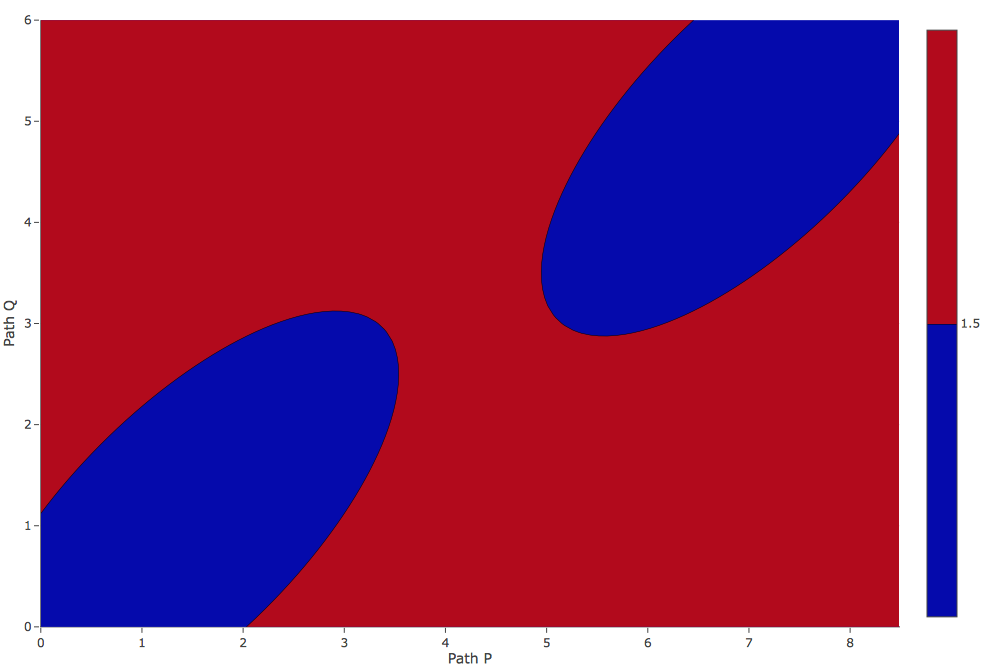
\includegraphics[width=0.27\textwidth]{freespace_lower.png} }}
    \qquad
    \subfloat[$\epsilon = \epsilon_F$]{{
    	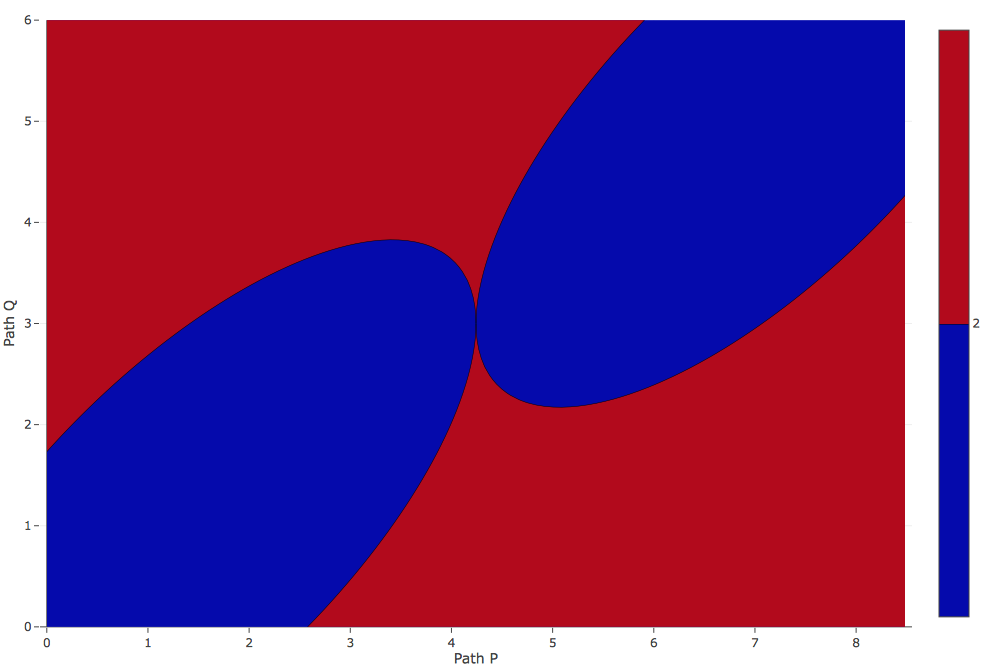
\includegraphics[width=0.27\textwidth]{freespace_eq.png} }}
    \qquad
    \subfloat[$\epsilon > \epsilon_F$]{{
		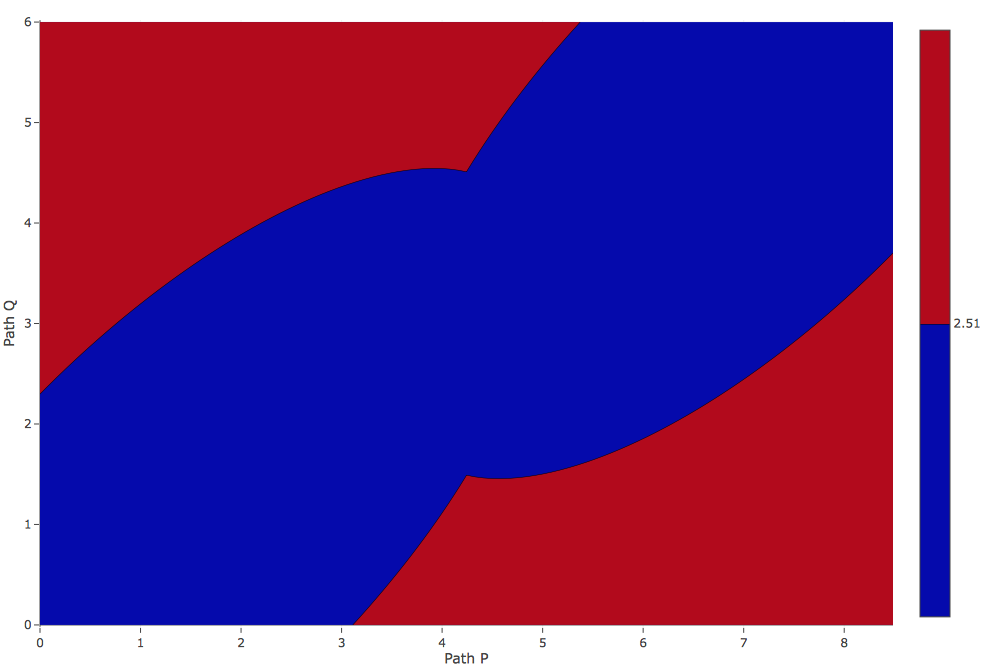
\includegraphics[width=0.27\textwidth]{freespace_higher.png} }}
	\caption{Three free-space diagrams with same height function $\delta$\protect\footnotemark}
    \label{fig:freespace_decision}
\end{figure}

\footnotetext{View the example here: \url{https://abegehr.github.io/frechet/?p=(1_2)(4_5)(7_2)&q=(1_3)(7_3)}}

The following cases are depicted in Figure \ref{fig:freespace_decision} above:
\begin{enumerate}[label=(\alph*)]
	\item $\epsilon$ is smaller than the Fréchet distance $\epsilon_F$. The decision algorithm returns false.
	\item $\epsilon$ is equal to the Fréchet distance $\epsilon_F$. The decision algorithm returns true.
	\item $\epsilon$ is larger than the Fréchet distance $\epsilon_F$. The decision algorithm returns true.
\end{enumerate}


\subsection{Classical Critical Events}

Alt and Godau also identified that the critical height $\epsilon_F$ where a critical pathway in the free-space diagram closes occurs in one of three cases. These are the three types of classical critical events:

\begin{enumerate}[label=(\alph*)]
	\item $\epsilon_F$ at $(0, 0) \in F_\epsilon$ or $(L_P, L_Q) \in F_\epsilon$
	\item A new passage with height $\epsilon_F$ opens on the border between two cells.
	\item A new horizontal or vertical passage with height $\epsilon_F$ opens on borders with cells in between.
\end{enumerate}

In Figure \ref{fig:classical_critical_events} example free-space diagrams for each type of classical critical event are shown.

\begin{figure}[H]
    \centering
    
    \subfloat[type a\protect\footnotemark]{{
		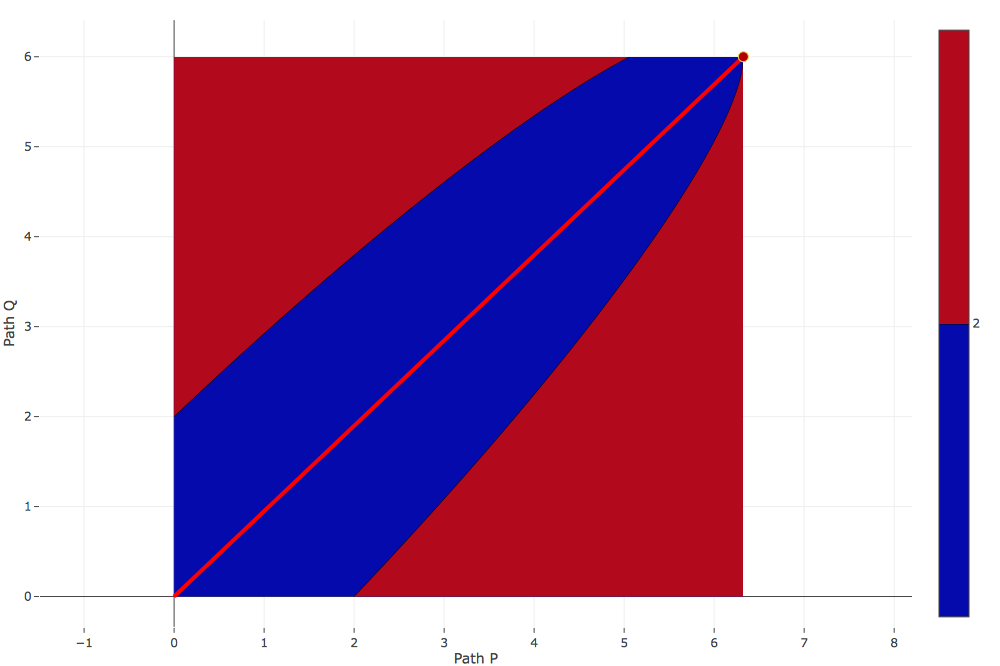
\includegraphics[width=0.27\textwidth]{classical_critical_event_a.png} }}
    \qquad
    \subfloat[type b\protect\footnotemark]{{
    	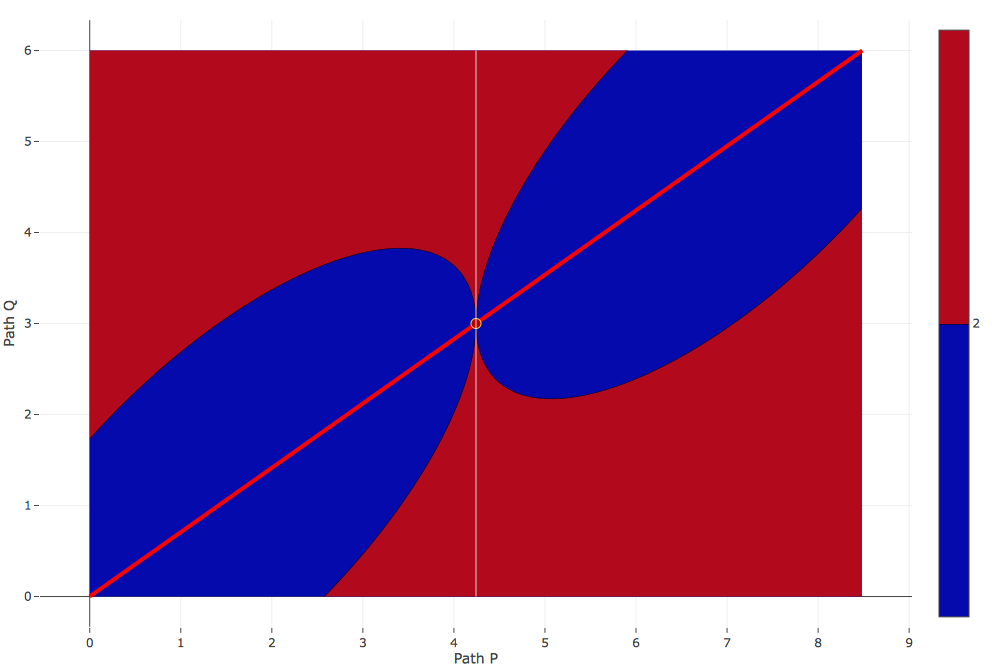
\includegraphics[width=0.27\textwidth]{classical_critical_event_b.png} }}
    \qquad
    \subfloat[type c\protect\footnotemark]{{
		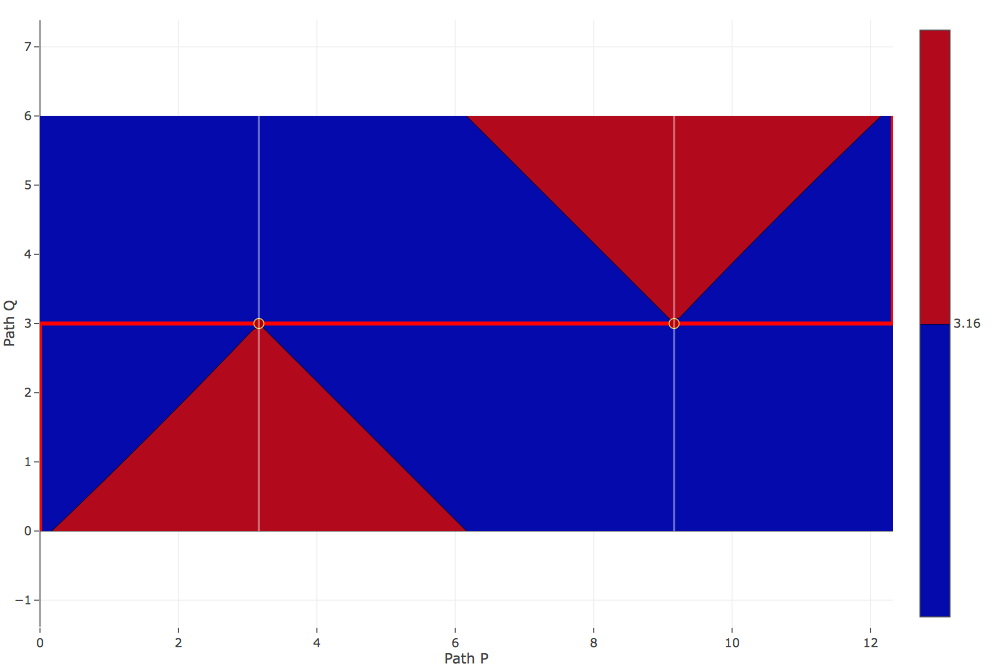
\includegraphics[width=0.27\textwidth]{classical_critical_event_c.png} }}

	\caption{Examples for the three types of classical critical events}
    \label{fig:classical_critical_events}
\end{figure}

\addtocounter{footnote}{-3} %3=n
\stepcounter{footnote}\footnotetext{Classical critical event of type a at height $\epsilon_F$ is at the upper-right corner $(L_P, L_Q)$. View the example here: \url{https://abegehr.github.io/frechet/?p=(1_3)(7_5)&q=(1_3)(7_3)}}
\stepcounter{footnote}\footnotetext{Classical critical event of type b at height $\epsilon_F$ is at vertical border connecting the left to the right cell. View the example here: \url{https://abegehr.github.io/frechet/?p=(1_2)(4_5)(7_2)&q=(1_3)(7_3)}}
\stepcounter{footnote}\footnotetext{Classical critical event of type c at height $\epsilon_F$ is at vertical border connecting the left to the right cell over the middle cell. View the example here: \url{https://abegehr.github.io/frechet/?p=(4_3)(7_4)(1_4)(4_3)&q=(1_3)(7_3)}}

Critical events will be denoted with $C_k$ where $C_k.A$ is the startpoint and $C_k.B$ is the endpoint. For classical critical events of type a or b the startpoint and endpoint are the same.


\subsection{Computing the Classical Fréchet Distance}

We now have the tools to compute the classical Fréchet distance. To compute the classical Fréchet distance, we can apply \textit{Algorithm 2} of \citeauthor*{altgodau}'s paper.\cite{altgodau} The algorithm first determines all classical critical events of type a, b, and c, including their critical $\epsilon$. Then using a binary search and the decision algorithm \textit{Algorithm 2} finds the smallest critical $\epsilon$ for which the height function $\delta$ is traversable.


\section{Lexicographic Fréchet Matchings}

In his \citeyear{rotelex} paper \citetitle{rotelex}, \citeauthor{rotelex} extended upon the findings from \citeauthor*{altgodau} in their paper \citetitle{altgodau} to establish an algorithm that produces a lexicographic Fréchet matching.

Taking a lexicographic approach roughly means that we want to minimise the time $T(s)$ during which the height exceeds a threshold $s$.\cite{rotelex} We want to spend as little time as possible at the current height and want to descend as quickly as possible.

\subsection{Steepest Descent}

To achieve a lexicographically optimised traversal, \citeauthor{rotelex} makes use of the steepest descent. Therefore he developed a steepest descent algorithm.

Because we chose our input to be two paths consisting of straight line segments, the level set in a cell consists of concentric ellipses. \citeauthor{rotelex} defines two lines for every cell, $l$ and $l'$:

\begin{itemize}
	\item [($l$)] The points where the ellipses have vertical tangents and $\delta$ has a linear horizontal gradient lie on line $l$ through the common center.\cite{rotelex}
	\item [($l'$)] The points where the ellipses have horizontal tangents and $\delta$ has a linear vertical gradient lie on line $l$ through the common center.\cite{rotelex}
\end{itemize}

Depending on whether we are descending from a point on one of the lines or from in between one of the quadrants they span up, the direction of the steepest descent is affected. Consult \citeauthor{rotelex}'s paper \citetitle{rotelex}\cite{rotelex} (Figure 5) for more detail. It is important to note at this point that the steepest descent for a point is unique.


\subsection{New Lexicographic Type of Critical Event}

\citeauthor{rotelex} also identifies a new lexicographic type of critical event which does not influence the global Fréchet distance $\epsilon_F$, but is essential for achieving a lexicographically correct traversal.

The new lexicographic type of critical event occurs while descending on a steepest descent path. It occurs when we would horizontally or vertically surpass a critical opening of the height at which we currently are.

Figure \ref{fig:new_critical_event} shows a minimal example of these new lexicographic types of critical events.

\begin{figure}[H]
    \centering
    
	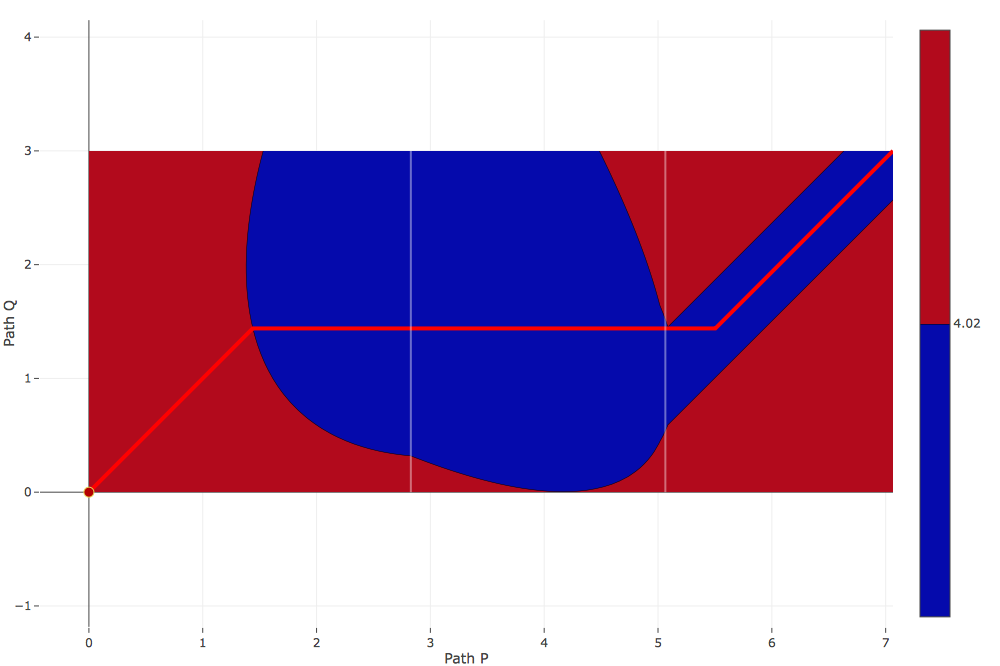
\includegraphics[width=0.7\textwidth]{new_critical_event.png}
	
	\caption{Example of new lexicographic type of critical event\protect\footnotemark}
    \label{fig:new_critical_event}
\end{figure}
\footnotetext{New lexicographic critical event of type a below height $\epsilon_F$ connects the middle of the left cell to the vertical border between the middle and the right cell. View the example here: \url{https://abegehr.github.io/frechet/?p=(3_2)(5_4)(3_3)(5_3)&q=(2_7)(5_7)}}


\subsection{Lexicographic Fréchet Matching Algorithm}\label{sec:lex_frechet_alg}

We now have the tools needed to understand \citeauthor{rotelex}'s algorithm for lexicographic Fréchet matchings\cite{rotelex} under \textit{general inputs} (not yet regarding degenerate inputs, as will be discussed in section \ref{lex_frechet_deg}). In contrary to the algorithm for computing the classical Fréchet distance, the algorithm for lexicographic Fréchet matching utilises recursion to result in a local traversal that is lexicographically optimised. The algorithm as described here is aligned to the implementation of the online visualisation.

\begin{algorithm}[H]
\caption{Requirements for Lexicographic Fréchet Matching Algorithm}\label{alg:lex_frechet_alg_req}
\begin{algorithmic}[1]

\Function{DecisionAlgorithm($\delta, A, B, \epsilon$)}{}
	\State \Comment{Implementation of the decision algorithm that decides if $\delta$ is traversable from $A$ to $B$ with $\epsilon$.}
	\State \Return {$true$ or $false$}
\EndFunction

\State {}

\Function{SteepestDescent($\delta, A, B, \epsilon_A, \epsilon_B$)}{}
	\State \Comment{Attempts a steepest descent as far as possible for the higher of $A$ and $B$, or both in case they reside at equal height. Attempt the steepest descent to $A'$ and $B'$ until $A'$ or $B'$ reaches a cell border or a line $l$ or $l'$, they would pass each other vertically or horizontally, or they meet each other. Descend to an equal height if possible.}
	\State \Return {$A', B', \epsilon_{A'}, \epsilon_{B'}$}
\EndFunction

\State {}

\Function{ReverseDescent($\delta, A, B, \epsilon_A, \epsilon_B$)}{} 
	\State \Comment{Reverses steepest descent until a classical critical event of type b or c, or a new lexicographic critical event is found. Also returns the critical event $c$.}
	\State \Return {$A', B', \epsilon_{A'}, \epsilon_{B'}, c$}
\EndFunction

\State {}

\Function{ClassicalFréchet($\delta, A, B, \epsilon_A, \epsilon_B$)}{} 
	\State \Comment{Using a binary search and the decision algorithm, this function finds the lowest traversable classical critical event that is needed to traverse $\delta$ from $A$ to $B$. This is the same as the algorithm for the classical Fréchet distance.}
	\State \Return {$\epsilon_F, c$}
\EndFunction

\end{algorithmic}
\end{algorithm}



\begin{algorithm}[H]
\caption{Lexicographic Fréchet Matching Algorithm}\label{alg:lex_frechet_alg}
\begin{algorithmic}[1]

\Function{TraverseRecursive($\delta, A, B, \epsilon_A, \epsilon_B$)}{}

	\If {$A = B$ \textbf{or} $B.x \leq A.x$ \textbf{or} $B.y \leq A.y$ }
		\State \Comment{Traversal done. Connect A and B.}
		\State \Return \Call{Connect}{$A, B$}
	\EndIf
	
	\State {$\epsilon \gets \max(\epsilon_A, \epsilon_B)$}
	
	\If {\Call{DecisionAlgorithm}{$\delta, A, B, \epsilon$}}
	
		\State $A', B', \epsilon_{A'}, \epsilon_{B'} \gets$ \Call{SteepestDescent}{$\delta, A, B, \epsilon_A, \epsilon_B$}
		
		\State {$\epsilon' \gets \max(\epsilon_{A'}, \epsilon_{B'})$}
		
		\If {\Call{DecisionAlgorithm}{$\delta, A', B', \epsilon'$}}
			\State \Comment{Traversable after steepest descent.}
			
			\State \Return \Call{TraverseRecursive}{$\delta, A', B', \epsilon_{A'}, \epsilon_{B'}$}
		
		\Else \Comment{Not traversable. The descent passes a critical event.}
		
		\While {$A \neq A'$ \textbf{or} $B \neq B'$}
		
			\State {$A', B', \epsilon_{A'}, \epsilon_{B'}, c \gets$ \Call{ReverseDescent}{$\delta, A', B', \epsilon_{A'}, \epsilon_{B'}$}}
			\State {$\epsilon' \gets \max(\epsilon_{A'}, \epsilon_{B'})$}
			
			\If {\Call{DecisionAlgorithm}{$\delta, A', B', \epsilon'$}}
				\State \Comment{Traversable with the critical event $c$.}
			
				\State \Return \Call{TraverseRecursive}{$\delta, A', c.B, \epsilon_{A'}, \epsilon_{c}$} $+$ $c$ $+$ \Call{TraverseRecursive}{$\delta, c.A, B', \epsilon_{c}, \epsilon_{B'}$}
			\EndIf
		
		\EndWhile
		
		\EndIf 
		
	\Else \Comment{A critical event with $\epsilon_c > \epsilon$ is needed to traverse.}
		
		\State $\epsilon_F, c \gets$ \Call{ClassicalFréchet}{$\delta, A, B, \epsilon_A, \epsilon_B$}
		
		\State \Return \Call{TraverseRecursive}{$\delta, A', c.B, \epsilon_{A'}, \epsilon_{c}$} $+$ $c$ $+$ \Call{TraverseRecursive}{$\delta, c.A, B', \epsilon_{c}, \epsilon_{B'}$}
	
	\EndIf
	
\EndFunction

\end{algorithmic}
\end{algorithm}


 